
% ページフォーマットの指定
\documentclass[twocolumn]{jsarticle}

  % 外部パッケージの導入
  % 引用
  \usepackage{cite}
  % 画像の出力
  \usepackage[dvipdfmx]{graphicx}
  
  % 画像元のパスの追加
  \graphicspath{{figure/}}
  
  % 文書本体の記述
  \begin{document}
  \title{プログレスレポート}
  \date{\today}
  \author{森健一郎\\配布対象:安藤先生}
  
  \maketitle
  
  \section{研究目的}
  プロセッサ・チップ上には,ホット・スポットと呼ばれる単位面積あたりの電力が大きい場所が存在する.ホット・スポットは,そうでない場所と比べて温度上昇が激しいため,プロセッサの故障を引き起こす可能性が高い.~\cite{Weste2010,Monsieur2001,Khan2010,Black1969,Viswanath2000}従って,ホット・スポットを生成する回路の消費電力を低下させる必要がある.

  ホット・スポットを生成する回路の1つに,発行キュー(IQ:issue queue)がある.IQ のサイズはプロセッサの世代が進むごとに大きくなっており,より深刻なホット・スポットとなっている.従って,IQ の電力削減に対する要求は非常に大きい.
  
  IQ の中で最も電力を消費するのは,タグ比較の回路である.タグ比較は,発行幅分のディスティネーション・タグとすべてのソース・タグで行われるため,電力効率が非常に悪い.そこで本研究では,ディスティネーション・タグとソース・タグの下位ビットが等しい命令についてのみ比較器を動作させることにより,動作する比較器の数を減少させ電力を削減する方法を提案する.

  提案手法は,次のように実現する.IQ を複数のセグメントに分割し,第 n セグメントには,第 1 ソース・タグの下位ビットが n である命令のみをディスパッチする.そして,ウェイクアップのタグ比較の際には,ディスティネーション・タグの下位ビットが,自身に割り当てられた命令の第1ソース・タグの下位ビットと等しいセグメントのみ,比較器を動作させてタグ比較を行う.この方法により,第1ソース・タグについての比較器の動作回数を「1/セグメント数」に減少させることができる.

  提案手法における欠点として,セグメントが詰まることによる性能低下が挙げられる.あるセグメントに空きがない状態で,そのセグメントにディスパッチされる命令が現れた場合を考える.この場合,他のセグメントにディスパッチすることはできないため,該当のセグメントに空きが出るまでディスパッチを停止する必要があり,これは性能低下に繋がる.本研究では,この欠点に対する対応策を考え,性能低下が許容できる範囲内に収まるようにする必要がある.

  また,その他の欠点として,第2ソース・タグの比較器の動作回数は削減できないことなどが挙げられる.これらの欠点に対しても十分に検討し,提案手法における電力削減及び性能の変化について評価を行う.

  \section{経過}

  \subsection{前回の経過}
  \begin{itemize}
    \item 提案手法の修正及びその評価
    \item Swap方式の改良及びその評価
    \item レジスタ・フリーリストのセグメント化の修正及びその評価
  \end{itemize}
  \subsection{今回の経過}
  \begin{itemize}
    \item ROB のサイズによる提案手法への影響の調査
    \item Last Tag Prediction の実装及び評価
  \end{itemize}

  

  \section{活動報告}
  \subsection{言葉の訂正}
  前回のレポートで,reg1 がレディであるため,どのセグメントに割り当てても問題のない場合のことを「セグメント・フリー」と記述していたが,適切な表現ではないとのご指摘を頂いた.そこで,以降では「セグメント・フレキシブル」と表現することにする.

  \subsection{ROB のサイズによる提案手法への影響}
  現在想定しているプロセッサ構成では,発行キュー(IQ)がいっぱいになってストールする前に,リオーダ・バッファ(ROB)がいっぱいになってストールしている可能性があることがわかった.そこで今回は,ROB のサイズを大きくした場合の IQ の占有率及び,提案手法による性能低下と比較回数の削減を再測定した.

  \begin{table}[htb]
    \caption{プロセッサの基本構成}
    \footnotesize
    \center
      \begin{tabular}{l|l} \hline \hline
       Pipeline width & 8 instructions wide for each of \\
       & fetch, decode, issue, and commit \\
      % Reorder buffer & 256 entries \\
       IQ & 128 entries \\
       Load/Store queue & 128 entries \\
       % Physical registers & 256(int) + 256(fp) \\
       Branch prediction & 12-bit history 4K-entry PHT gshare \\
       & 2K-set 4-way BTB \\
       & 10-cycle misprediction penalty \\
       Function unit & 4 iALU, 2 iMULT, \\
       &  3 FPU, 2 LSU \\
       L1 D-cache & 32KB, 8-way, 64B line \\
        & 2-cycle hit latency \\
       L1 I-cache & 32KB, 8-way, 64B line \\
        &  2-cycle hit latency \\
       L2 cache & 2MB, 16-way, 64B line \\
        & 12-cycle hit latency \\  
       Main memory & 300-cycle latency \\
       & 8B/cycle bandwidth \\ 
       Prefetch & stream-based,32-stream tracked,  \\ 
       & 16-line distance, 2-line degree, \\
       & prefetch to L2 cache \\ \hline
    \end{tabular}
    \label{tab:base_config}
  \end{table}

  \begin{table}[htb]
    \caption{各評価モデルにおける ROB のサイズ}
    \footnotesize
    \center
      \begin{tabular}{l|l|l} \hline \hline
      model & Reorder buffer & Physical registers \\ \hline
      small & 256 entries & 256(int) + 256(fp) \\
      medium & 320 entries & 320(int) + 320(fp) \\
      huge & 1024 entries & 1024(int) + 1024(fp) \\ \hline
    \end{tabular}
    \label{tab:rob_size}
  \end{table}

  \subsubsection{評価環境及び評価モデル}
  \label{sec:config}
  評価環境について説明する.シミュレータには SimpleScalar をベースに修正を加えたものを使用した.表\ref{tab:base_config}にプロセッサ構成を示す. 
  
  測定ベンチマークには,SPEC CPU 2017 ベンチマークのうち,int 系 9 本と fp 系 9 本の計 18 本を使用した.ベンチマークの測定区間は,プログラムの先頭から 16G 命令をスキップした後の 100M 命令である.

  今回は ROB のサイズとして,表~\ref{tab:rob_size}に示すような 3 種類のモデルを用意した.small はこれまでの評価と同じサイズである.medium は Intel Skylake のプロセッサ構成における ROB と IQ のサイズ比を考慮して設定した. huge は,ROB によるつまりを起こさないような理想的なモデルである.

  なお,各モデルにおけるレジスタ・ファイルの数はROB のサイズと同じ値に調整してある.
  \begin{figure*}[ht]
    \centering
    \includegraphics[width=0.99\hsize]{occupency_rob.pdf}
    \caption{ROB のサイズが与える IQ の占有率への影響}
    \label{fig:occupency_rob}
  \end{figure*}

  \subsubsection{ROB のサイズと IQ の占有率}
  ROB のサイズを変化させた場合の IQ の占有率を測定した.なお,本測定での IQ の方式は,エイジ論理付きのランダム・キューである.測定結果を,図 ~\ref{fig:occupency_rob}に示す.

  図より,いくつかのベンチマークで,発行キューの占有率が大きく増加していることが分かる.特に,xalancbmk,bwaves, cactuBSSN,lbm, imagick,roms で顕著である.これらのベンチマークにおいては,small では先に ROB が詰まっていたのが,medium や huge で ROB の詰まることがなくなった結果,IQ の占有率が大きく上昇したと考えられる.
  
  以降の評価では,ROB が与える提案手法への影響を排除するため,huge モデルの ROB を使用して評価を行う.
  
  \begin{figure*}[ht]
    \centering
    \includegraphics[width=0.99\hsize]{ipc_rob.pdf}
    \caption{提案手法における性能変化(hugeモデル)}
    \label{fig:ipc_rob}
  \end{figure*}

  \begin{figure*}[ht]
    \centering
    \includegraphics[width=0.99\hsize]{reduction_rob.pdf}
    \caption{提案手法における比較器の動作回数削減(hugeモデル)}
    \label{fig:reduction_rob}
  \end{figure*}

  \begin{figure*}[ht]
    \centering
    \includegraphics[width=0.99\hsize]{occupency.pdf}
    \caption{提案手法における占有率の変化(hugeモデル)}
    \label{fig:occupency}
  \end{figure*}

  \subsubsection{huge モデルの場合の提案手法の再評価}
  \label{sec:hyouka}
  ROB の詰まりがおきない huge モデルにおいて,提案手法の再評価を行った.評価結果を図~\ref{fig:ipc_rob},~\ref{fig:reduction_rob},~\ref{fig:occupency}に示す.
  図における normal は,スワップを全く行わない提案手法であり,swap は,前回レポートでの SWAP\_CONSERVATIVE モデルに STDS を適応した,最も占有率が低下しないような提案手法のモデルである.なお,セグメントの分割数は 16 としている.以下で,これまでの測定と大きく変化のあった性能低下に関して詳しく考察する.なお,占有率と比較器の動作回数削減に関しては前回の評価とほとんど同様であるため省略する.
  
  \paragraph{性能低下}まず,図~\ref{fig:ipc_rob}の性能低下に関して考える.今回の結果では,normal の場合に,これまでの評価で見られなかった性能低下がいくつかのベンチマークで見られていることが分かる.xalancbmk, cactuBSSN, lbm, roms などが挙げられる.
  
  これらのベンチマークは,small から huge にした際に占有率の上昇が大きかったベンチマークと一致する.またこれらのベンチマークは,前回のレポートで示した,容量効率が重要なベンチマークにも該当している.したがって,これらのベンチマークでは,提案手法によって IQ の容量効率が低下し,それが原因で性能が低下していると言える. 

  次に swap の結果に関して考える.swap の場合,すべてのベンチマークで大きな性能低下は見られない.従って,容量効率を重視した方式によって,占有率の低下を防ぐことができ,結果として大きな性能低下を防ぐことができている.図~\ref{fig:occupency} を見ても,normal と比較して swap では占有率が高く,比較的 base に近い値を示していることが分かる.

  \subsubsection{ここまでの評価のまとめ}
  前回のレポートと,今回の再評価の結果についてまとめる.
  \begin{itemize}
    \item これまでの評価で性能がほとんど低下していなかったのは,ROB のサイズが IQ のサイズに対して不十分で,ROB が先に詰まるという現象が生じていたため.
    \item 上記の問題を解消して測定した結果,IQ の容量効率が重要なベンチマークでは提案手法によって 5\% から 10\% 程度性能が低下した.
    \item 容量効率を重要視したモデルの提案手法を使用することによって,IQ の容量効率を低下させず,性能に影響を与えないことが可能である.本手法によって,比較器の動作回数を平均で60\% 削減することができる.
  \end{itemize}

  \subsection{Last Tag Prediction の実装及び測定}
  前回のレポートで,提案手法において第 1 ソース・レジスタ(reg1)と第 2 ソース・レジスタ(reg2)がともにレディでない場合で,なおかつ reg1 に該当するセグメントに空きがない場合に, スワップを行って reg2 によって割り当てるセグメントを決定する手法である,STDS(Selecting Tag to Decide Segment) を提案した.今回は,そのさらなる改良として,Last Tag Prediction を実装し,その評価を行った.
  
  \begin{figure}[ht]
    \centering
    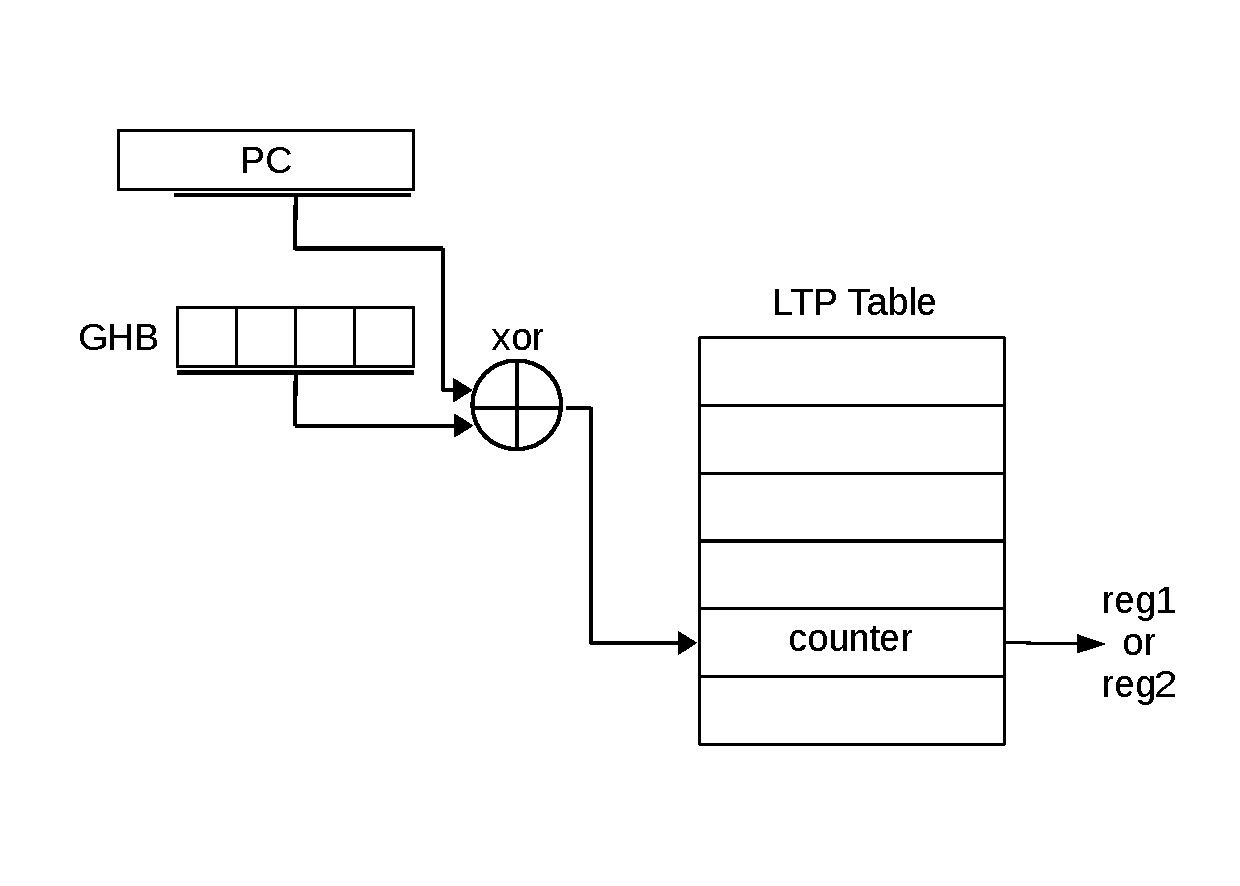
\includegraphics[width=0.99\hsize]{ltp.pdf}
    \caption{Last Tag Predictor}
    \label{fig:ltp}
  \end{figure}

  \subsubsection{Last Tag Prediction}
  reg1 と reg2 がともにレディでない場合は,両方のオペランドについてタグ比較が行われる.そこで,「よりレディとなるのが遅いオペランド」のタグ(ラスト・タグ)を,セグメント化した方に格納することによって,より比較回数を削減できると考えられる.ただし,どちらのオペランドがより後にレディになるかという情報は,ディスパッチ時にはわからないため,予測を行う必要がある.

  ラスト・タグの予測方法は,論文~\cite{ernst2002}で提案されている.この方法を Last Tag Prediction(LTP)と呼ぶ.以下,LTP について説明する.

  LTP は,図~\ref{fig:ltp}のように.命令の PC をインデクスとするテーブルで,テーブルの各エントリは2 ビットの飽和型アップ・ダウン・カウンタで構成される.このカウンタは,値が 0 または 1 の場合に reg1 がラスト・タグであることを示し, 2 または 3 の場合に reg2 がラスト・タグであることを示す.予測と学習の方法について説明する.
  
  \paragraph{予測}命令ディスパッチ時に,reg1 reg2 ともにレディでなく,なおかつ両方のタグに該当するセグメントに空きがある場合に,予測が行われる.PC を用いてテーブルを検索し,該当のカウンタの値を読み出すことによって行う.reg1 がラスト・タグであると予測された場合には,reg1 によって割り当てるセグメントを決定する.reg2 がラスト・タグであると予測された場合には,スワップを行い reg2 によって割り当てるセグメントを決定する.
  
  なお,reg1 reg2 ともにレディではないが,いずれかのタグに該当するセグメントに空きがない場合は,予測は行わずに空きのあるセグメントのほうに割当を行う.また,どちらのセグメントにも空きがない場合にはストールする.

  \paragraph{学習}
  学習は命令発行時に,ディスパッチ時に予測を行った命令でのみ行われる.reg1 と reg2 がレディとなったサイクルを比較し,reg1 のほうが遅い場合にはカウンタをデクリメントし,reg2 のほうが遅い場合にはカウンタをインクリメントする.

  \begin{figure*}[ht]
    \centering
    \includegraphics[width=0.99\hsize]{ltp_reduction.pdf}
    \caption{LTP を適応した提案手法による比較回数削減(hugeモデル)}
    \label{fig:ltp_reduction}
  \end{figure*}

  \begin{figure*}[ht]
    \centering
    \includegraphics[width=0.99\hsize]{ltp_accuracy.pdf}
    \caption{LTP の予測精度(hugeモデル)}
    \label{fig:ltp_accuracy}
  \end{figure*}

  \subsubsection{LTP の評価}
  LTP を用いた提案手法の評価結果を図~\ref{fig:ltp_reduction},~\ref{fig:ltp_accuracy}に示す.評価環境は~\ref{sec:config}節と同様である.使用している評価モデルは以下のとおりである.
  \begin{itemize}
    \item swap:SWAP\_CONSERVATIVE に STDS を適応したモデル.(\ref{sec:hyouka}節の swap と同じ)
    \item perfect:LTP において,完璧に予測できるとした理想的なモデル
    \item 1024 entries:LTP のテーブルが 1024 エントリであるモデル
    \item 4096 entries:LTP のテーブルが 4096 エントリであるモデル
  \end{itemize}

  まず,比較回数の削減から考える.図より,perfect では swap に比べて平均で 5\%p 程度削減率が向上していることが分かる. 特に,lbm や roms などでは 10\%p 弱削減率が増加している.従って,精度の高い予測を実現することができれば,LTP の効果は期待できると言える.

  しかし,1028 entries や 4096 entries と swap を比較すると,その増加率は平均で 2\%p 弱程度と, perfect ほどの削減ができていない.この理由は,図~\ref{fig:ltp_accuracy}に示した予測精度を見ることによって分かる.図より,LTP の予測精度は平均で65\% 程度となっており,これは予測器の精度としては大変低いと言える.従って,予測器の精度を上げなければ,LTP による追加の削減は期待できない.

  論文~\cite{ernst2002}によると,LTP のインデクスに PC と分岐履歴の xor を取ったものを用いる gshare style のほうが良いと記載されている.従って,今後の課題として,gshare style の LTP を実装して予測精度の向上を測ることが挙げられる.

  ただ,予測が完璧にできたとした場合でも,LTP による追加の削減は平均で 5\%p 程度であることと,予測器を実装するための追加のハードウェアや消費電力があることを考えると,LTP の有効性はそこまで高くないかもしれない.

  \section{研究計画}
  
  \begin{itemize}
    \item HSPAICE を用いた電力測定を開始する
    \begin{itemize}
      \item 測定方法などを松田さんから教わる
    \end{itemize}
    \item LTP のチューニングを行い予測精度を向上させる
    \begin{itemize}
      \item gshare style を実装する
      \item その他の予測方法がないか調べる
    \end{itemize}
  \end{itemize}
  
  \section{関連文献:Efficient Dynamic Scheduling Trough Tag Elimination~\cite{ernst2002}}
  本論文では,発行キューにおけるタグ比較器を削減するための手法として,発行キューを,1)オペランドが両方共レディな命令,2)オペランドが片方だけレディな命令,3)オペランドが両方レディでない命令専用の3つのブロックに分割する方法を提案している.1) の発行キューには比較器は必要なく,2) の発行キューには比較器は 1 つあれば良い.そして3) の場合のみ,従来と同じく 2 つの比較器が必要となる. 
  
  また,さらなる工夫として,3) の場合に,どちらのオペランドがラスト・タグとなるかを予測し,そちらのタグのみ比較を行うといった工夫をしている.今回は,この予測方式(Last Tag Prediction)に関して詳しく述べる.
  
  \subsection{Last Tag Prediction}
  Last tag Prediction は,基本的にレポート中に示したものと同様であるが,本論文ではさらに,テーブルのインデクスとしてPC とグローバルな分岐履歴との xor をとったものを使用して,分岐予測器における gshare の形式でインデクスを計算している.論文によると,グローバル履歴は 8 ビット程度が適切であるとされている.この予測器の予測精度は,1024 エントリで 8 割程度, 8192 エントリで 9 割程度である.

  % 参考文献
  \bibliographystyle{../Config/andolab2} 
  \bibliography{../Config/ref}
  
  \end{document}
  